\documentclass[UTF8]{ctexart}
\ctexset { section = { format={\Large \bfseries } } }
\pagestyle{plain}
\usepackage{float}
\usepackage{amsmath}
\usepackage{amssymb}
\usepackage{listings}
\usepackage{graphicx}%插入图片宏包
\usepackage{xcolor}
\usepackage{geometry}
\geometry{a4paper,scale=0.8}
\usepackage{caption}
\usepackage{subcaption}
\usepackage[linesnumbered,ruled]{algorithm2e}
\usepackage[colorlinks=true, linkcolor=blue, citecolor=blue, urlcolor=blue]{hyperref}
\captionsetup[figure]{name={Figure}}
\captionsetup[table]{name={Table}}
\definecolor{Rhodamine}{RGB}{227,11,92}

\lstset{
language=Python, % 设置语言
basicstyle=\ttfamily, % 设置字体族
breaklines=true, % 自动换行
keywordstyle=\bfseries\color{blue}, % 设置关键字为粗体,
morekeywords={}, % 设置更多的关键字,用逗号分隔
emph={self}, % 指定强调词,如果有多个,用逗号隔开
emphstyle=\bfseries\color{Rhodamine}, % 强调词样式设置
commentstyle=\color{black!50!white}, % 设置注释样式,斜体,浅灰色
stringstyle=\bfseries\color{red!90!black}, % 设置字符串样式
columns=flexible,
numbers=left, % 显示行号在左边
numbersep=2em, % 设置行号的具体位置
numberstyle=\footnotesize, % 缩小行号
frame=single, % 边框
framesep=1em % 设置代码与边框的距离
}

\title{\textbf{Data Structure lab8}}
\author{吴嘉骜 21307130203}
\date{\today}

\begin{document}

\maketitle

\noindent
\textbf {\large Experiment environment} \\
   Windows 11 VsCode Python 3.11.5 64-bit\\

\setlength{\parindent}{0pt}
\section*{Critical Paths}
The Program (or Project) Evaluation and Review Technique, commonly abbreviated PERT, 
is a statistical tool, used in project management, that is designed
to analyze and represent the tasks involved in completing a given project. First
developed by the United States Navy in the 1950s, it is commonly used in con-
junction with the critical path method or CPM.\\
Critical paths in PERT chart analysis: Edges represent jobs to be performed,
and edge weights represent the times required to perform particular jobs. If
edge $(u, v)$ enters vertex $v$ and edge $(v, x)$ leaves $v$, then job $(u, v)$ must be
performed prior to job $(v, x)$. A path through this dag represents a sequence of
jobs that must be performed in a particular order. A critical path is a longest
path through the dag, corresponding to the longest time to perform an ordered
sequence of jobs.\\
The PERT chart formulation given above is somewhat unnatural. It would be
more natural for vertices to represent jobs and edges to represent sequencing
constraints; that is, edge $(u, v, w)$ would indicate that job $u$ must be performed
before job $v$. Weights would then be assigned to edges. Write a
procedure that can finds a longest path in a directed acyclic graph with weighted edges.

\textbf{\large Solution}:\\
The code from \texttt{pert.py} is as follows:
\begin{lstlisting}
def toposort(graph):
    """
    Parameters:
        - graph: a dictionary representing a graph
        
    Returns:
        - a list of vertices in topological order
    """
    def dfs(v):
        # depth first search from vertex v
        visited.add(v)
        for u, _ in graph[v]:
            if u not in visited:
                dfs(u)
        result.append(v)

    visited = set()  # visited vertices
    result = []  # topological order of vertices

    for v in graph:
        if v not in visited:
            dfs(v)

    return result[::-1]  # reverse order

def dag_longest(graph):
    '''
    Parameters:
        - graph: a dictionary representing a graph
        
    Returns:
        - a list of vertices in the longest dist, and the length of the dist
    '''
    # Perform a Topological Sort on the graph
    topo_order = toposort(graph)
    # Initialize the maximum distance and corresponding dist
    max_dist = float('-inf')
    longest_path = []
    # Check each vertex as a starting point
    for s in topo_order:
        # Initialize the distance to each vertex to be -inf and the parent to be None
        dist = {v: (float('-inf'), None) for v in graph}
        dist[s] = (0, None)
        # Relax each edge in the topological order
        for v in topo_order:
            for u, w in graph[v]:
                if dist[v][0] + w > dist[u][0]:
                    dist[u] = (dist[v][0] + w, v)
        # Find the vertex with the largest distance from s
        max_dist_cur = max(dist.values(), key=lambda x: x[0])[0]
        # Update the maximum distance and corresponding dist
        if max_dist_cur > max_dist:
            max_dist = max_dist_cur
            max_v = max(dist, key=lambda x: dist[x][0])  # the vertex with the largest distance from s
            path_tmp = []
            while max_v:
                path_tmp.append(max_v)
                max_v = dist[max_v][1]
            longest_path = path_tmp[::-1]
    
    return longest_path, max_dist
\end{lstlisting}
\textbf{\large Interpretation}:\\
The \texttt{toposort} function performs a topological sort on the graph, 
and the \texttt{dag\_longest} function finds the longest path in the graph.\\
The idea of the algorithm is similar to a DAG single-source shortest path algorithm, which is based on the topological sort of the graph.
The difference is that we have to check each vertex as a starting point, and find the vertex with the largest distance from the starting point.
The inner loop of the algorithm relaxes each edge in the topological order, and updates the distance and predecessor of each vertex.\\
The pseudocode of the algorithm is as follows:\\
\begin{algorithm}[H]
  \SetAlgoLined
  \KwResult{The longest path in a DAG with weighted edges}
  \textbf{Input:} A directed acyclic graph \( G = (V, E) \) with a weight \( w(u, v) \) for each edge \( (u, v) \in E \)\;
  Perform a topological sort on \( G \)\;
  \For {each vertex \( s \) as a starting point} {
    \textbf{Initialization:} Set \( longestPath(v) = -\infty \) for each vertex \( v \), except for the start vertex $s$ which is set to 0. Create an array \( predecessors \) to store predecessors\;
    \For {each vertex \( v \) in topological order} {
      \For {each edge \( (v, u) \) in \( E \)} {
        \If{\( longestPath(u) + w(u, v) > longestPath(v) \)}{
          Update \( longestPath(v) = longestPath(u) + w(u, v) \)\;
          Update \( predecessors[v] = u \)\;
        }
      }
    }
  }
  Find the end vertex \( v \) with the maximum value in \( longestPath \)\;
  Reconstruct the path from the end vertex \( v \) using \( predecessors \) and determine the length\;
  \textbf{Output:} The longest path and its length\;
  
  \caption{Algorithm for finding the longest path in a DAG with weighted edges}
\end{algorithm}
\textbf{\large Results}:\\
We test the algorithm on the examples in Figure \ref{fig:examples}. The answers are correct, and note that there may be multiple longest paths in a graph.\\
\begin{figure}[htbp]
  \centering
  \begin{subfigure}{0.3\textwidth}
      \centering
      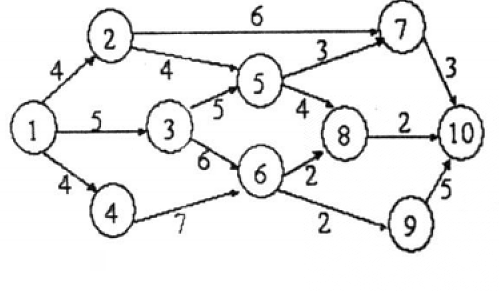
\includegraphics[width=\linewidth]{example1.png}
      \caption{Example Graph 1}
  \end{subfigure}%
  \hfill
  \begin{subfigure}{0.3\textwidth}
      \centering
      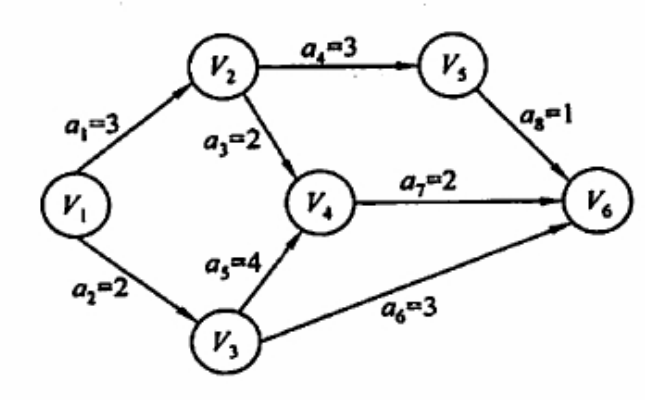
\includegraphics[width=\linewidth]{example2.png}
      \caption{Example Graph 2}
  \end{subfigure}%
  \hfill
  \begin{subfigure}{0.3\textwidth}
      \centering
      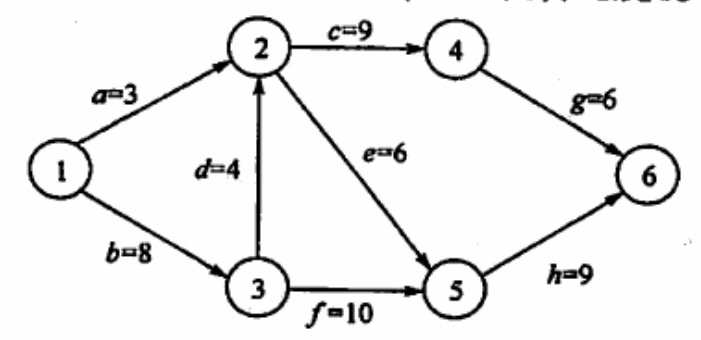
\includegraphics[width=1.2\linewidth]{example3.png}
      \caption{Example Graph 3}
  \end{subfigure}%
  \vspace{0.5cm}
  \begin{subfigure}{0.5\textwidth}
    \centering
    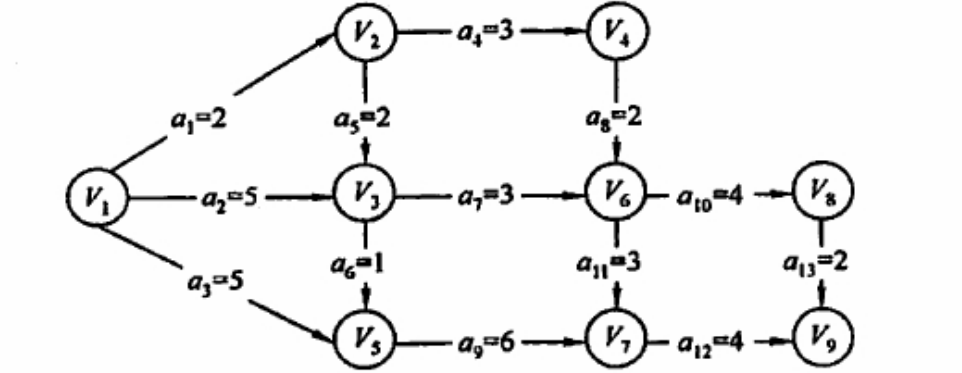
\includegraphics[width=0.8\linewidth]{example4.png}
    \caption{Example Graph 4}
  \end{subfigure}%
\begin{subfigure}{0.5\textwidth}
  \centering
  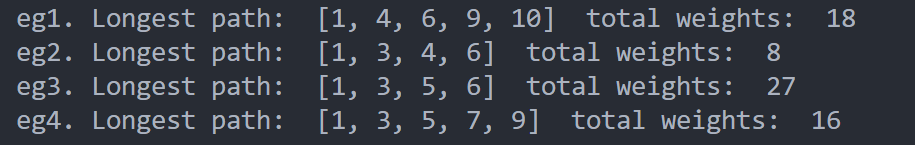
\includegraphics[width=\linewidth]{eganswer.png}
  \caption{Output of the answers}
  \end{subfigure}%
  \caption{Examples of DAGs and their longest paths}
  \label{fig:examples}
\end{figure}

\textbf{\large Complexity Analysis}:\\
To analyze the complexity of the algorithm above, we can consider the following components:

\begin{enumerate}
    \item \textbf{Topological Sort}: The topological sort of a graph \( G = (V, E) \) has a complexity of \( O(V + E) \), as it requires visiting every vertex once and examining all edges once.

    \item \textbf{Main loop}: The main loop of the algorithm iterates over all vertices \( V \) as a starting point. Then for each vertex, it iterates over all edges \( E \) to relax them. Therefore, the complexity of the main loop is \( O(V \cdot (V+E)) \).

    \item \textbf{Finding the Longest Path}: Finding the vertex with the maximum distance takes \( O(V) \), and tracing the longest path takes \( O(V) \) in the worst case.
\end{enumerate}

Therefore, the overall complexity of the algorithm is \( O(V^2+V \cdot E) \).

In most cases, \( O(V \cdot E) \) will be the dominating term, except for very sparse graphs where \( O(V^2) \) might be comparable.\\ 
\end{document}